\documentclass[11pt]{article}
\usepackage{amsmath}
\usepackage{mathtools}
\usepackage{txfonts}
\usepackage[margin=1.0in]{geometry}
\usepackage{graphicx}
\usepackage{float}
\usepackage{booktabs}
\usepackage[caption=true]{subfig}
\graphicspath{ {images/} }
\usepackage{appendix}
\usepackage{url}
%\usepackage{wrapfig}
\usepackage{algorithm}
\usepackage[noend]{algpseudocode}
\usepackage{caption}


\setlength{\parskip}{\baselineskip}%
\setlength{\parindent}{0pt}%
\renewcommand{\baselinestretch}{1.4}

\title{A regression model for predicting rail transit ridership at the station level}
\author{Daniel Hartig}
\date{\vspace{-5ex}}

\DeclareMathOperator*{\argmin}{arg\,min}


\begin{document}
\maketitle

\section{Introduction}

The United States is undergoing a rail boom. Since 2010, new light rail lines have opened in Dallas, Los Angeles, Salt Lake City, Denver, Minneapolis, Houston, Seattle and more.  A new heavy rail line opened in Washington DC, and a commuter rail system in Orlando. As transit expands in cities in the United States, there is an opportunity to validate predictive rail ridership models. 

A survey of transit agencies \cite{Boyle2006} conducted by the Transit Cooperative Research Program showed that relatively few agencies are using quantitative models when forecasting ridership for new lines, extensions or stations under consideration for funding. Of the 35 agencies that responded to the survey, 29 use professional judgment and 28 use rules of thumb among one or more techniques used to generate ridership forecasts. Another method used by 22 agencies is service elasticity; a set of general transit demand response curves for changing transportation options, published by the Transportation Research Board \cite{tcrp95}. 

For quantitative methods, the most commonly used technique--by 18 of 35 surveyed agencies--is the four-step travel demand model \cite{McNally2008}, introduced by Mannheim and Florian \cite{Mannheim1979, Florian1988}. The Mannheim-Florian model's four steps are trip generation, trip distribution, mode choice and route choice. In the trip generation phase, trip endpoints are created with as production and attraction ends. In the trip distribution step, these endpoints are paired up to generate trips; for example a residence with a a job, or hotel with a tourist attraction. In the mode choice step, trips are assigned to various transportation modes, such as personal vehicle, bus, or walking. Finally, in the route choice step, a route using that mode of transportation is chosen.

An implementation of the Mannheim-Florian model can be seen in the Seattle's Sound Transit Ridership Forecasting Methodology Report \cite{ST3_2015, ST3_add}. The Sound Transit 3 (ST3) was a ballot measure that passed in 2016 for a \$54 billion expansion of the local light rail system involving 100 km of new tracks and 37 new stations. The ridership forecasting methodology report explained how the project's official ridership projections were developed. The regional area is divided into 785 Alternatives Analysis Zones and for each of these zones transit surveys and recorded ridership on local bus routes were used to complete the trip generation and trip distribution steps. The mode choice and route choice is done using an incremental logit model to predict changes in transit mode based on changes in transit mode availability.

Only seven of the 35 surveyed agencies used regression models to predict future transit ridership. This thesis proposes a regression-based model using data from the United States Census Bureau at the zip code level. The model will be trained on the zip code characteristics and ridership data from existing light and heavy rail transit systems and used to predict ridership on other rail transit systems.  

\subsection{Original Contributions}

There are two main objectives of this thesis. The first objective is to investigate the utility of various data from the US Census Bureau as predictor variables in a regression model for urban rail ridership. The second objective is to determine what regression methods--loss functions and link functions--are best suited to modeling urban rail ridership given the available data.

This thesis diverges from previous regression modeling by investigating an expanded set of potential features. The US Census Bureau provides extensive data on a per-zip code bases as detailed in Section \ref{sec:data}, there are over a thousand possible data points available. This data is provided as counts per zip code. To translate this zip code data into features for a regression model, this thesis presents a novel geographic sampling method in Section \ref{sec:sampling}. 

With features for regression analysis in hand, this thesis tests several different regression methods against each other. Previous regression based analyses of urban rail ridership have exclusively used ordinary least squares regression. This thesis expands the model base to include other loss functions and link functions and reports accuracy metrics for each model. 

\section{Data Sources and Feature Generation}

\subsection{Selection of Transit Systems}

The response variable for the regression analysis is average weekday ridership over a period of at least one year. Ridership data for agencies that publish annual ridership reports is used to validate the model (for ridership data sources, see Appendix \ref{app:ridership}). Six cities were selected for this study: Boston, Chicago, Los Angeles, Atlanta, Dallas, and Denver. Several cities were eliminated from analysis for various reasons. A limitation of the dataset is that it does not include government employment. While state level employment is significant in all potential cities, state employment levels are relatively constant from city to city. Federal employment varies greatly, however; Washington DC had to be eliminated due to the large impact of un-recorded federal employment. San Francisco and Philadelphia were eliminated because they have multiple rail systems without integrated fares. New York City was eliminated because its subway has higher ridership than all other intra-urban rail systems in the country combined.

Ridership data is captured by different methods in different cities, but the same underlying data is counted by each case. In Chicago and Boston, station entrances are measured, and Boston additionally reports transfers between lines at each transfer station. Therefore, daily ridership is measured as the total number of entrances per station per day. This results in one count per one trip; and two counts per one daily commute. Dallas, Denver and Los Angeles report boarding and alighting by train car; so daily ridership is measured as the total number of boardings per stations per day. For transfer stations, boarding is `double counted' since a boarding at station A and a transfer at station B would result in two counts per one trip. Therefore, for these three networks, the transfer stations and their unusually high ridership counts are excluded from the analysis. For Atlanta, the ridership reporting definition is unknown, so we eliminate the transfer stations to be safe. For Boston and Chicago, ridership is counted by extracting data from the fare system for paid station entries. In Dallas and Denver, passenger counts are measured at the train car by Automated Personnel Counters. In Los Angeles and Atlanta the counting methodology is unknown. 

The data closest to 2015 is used when possible to get an accurate relation between ridership and census data. The census data as well as Chicago, Dallas, and Denver's ridership statistics are from 2015. Boston's ridership is from 2014, Los Angeles' is from 2013-2014, and Atlanta's is from 2010-2013. 

\subsection{Data Sources for Predictor Variables}\label{sec:data}

The zip code level data for feature generation comes from the US Census Bureau and is available at \texttt{factfinder.census.gov}. There are thousands of potential data sets available. We refer to the data points available for each zip code as characteristics of the zip code. Selection of features is guided by Kuby \cite{Kuby2004}, Taylor \cite{Taylor2008}, and Currie \cite{Currie2011}, who demonstrate the significance of characteristics such as employment, population, universities, poverty, airports, park and ride stations, and rental housing units. The characteristics can be divided into two categories: counting characteristics and dummy variables. 

This model emphasizes using only features that have `real' units, as opposed to binary features. The only binary dummy variable this model uses as a feature is for the presence of park-and-ride parking spaces at a transit station. Instead of using measures of land use mix as proposed in other models \cite{Durning2015, Gutierrez2011}, or binary dummy variables for universities and central business districts, the equivalent information is provided naturally as counting data in the feature set. Counts of housing types (such as large apartment buildings versus single family homes) replace land use mix; the number of jobs at universities or in financial jobs provide more information than dummy variables for presence of universities or central business districts. 

\begin{table}[H]
\centering\begingroup\fontsize{10}{10}\selectfont
\begin{tabular}{ll}
\toprule \textbf{Population related}&\textbf{Employment related} \\ 
\midrule Total population&Total Employment pay\\
Population over age 65& Employment in finance industry\\
Population with bachelor's degree& Employment at hospitals\\
Number of residents employed full time&\\
Number of housing units built after 2000&\\
\bottomrule
\end{tabular}\endgroup
\caption{Examples of characteristics associated with zipcodes}\label{tab:char}
\end{table}

The selected characteristics are generally related either to the population of the zip code or the number of jobs of the zip code. The captured characteristics of the built enviornment, such as the quantity, age, and building type of the housing stock, are generally related to population. For example, the total number of housing units is expected to be highly correlated with the population of a zip code.  Examples of characteristics are provided in Table \ref{tab:char}. Some characteristics, such as total population, are expected to have a positive relationship with ridership; others, such as population under the age of 18, are expected to have a negative relationship. Examples of associations between characteristics and ridership are provided in Figure \ref{fig:chartypes}. A summary of all the selected characteristics is provided in Appendix \ref{app:features}.



\begin{figure}[H]
\centering
\subfloat[Example of a positive relationship]{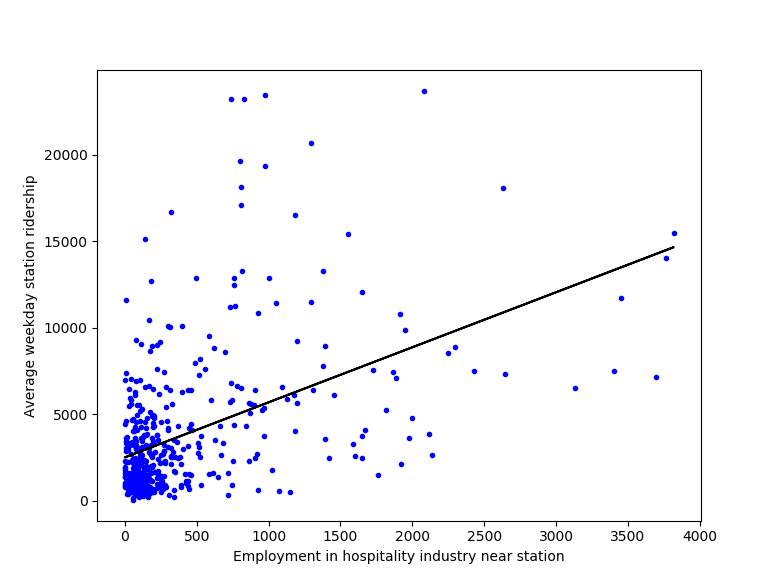
\includegraphics[clip,width=0.5\columnwidth]{exRegPosSlope}}
\subfloat[Example of a negative relationship]{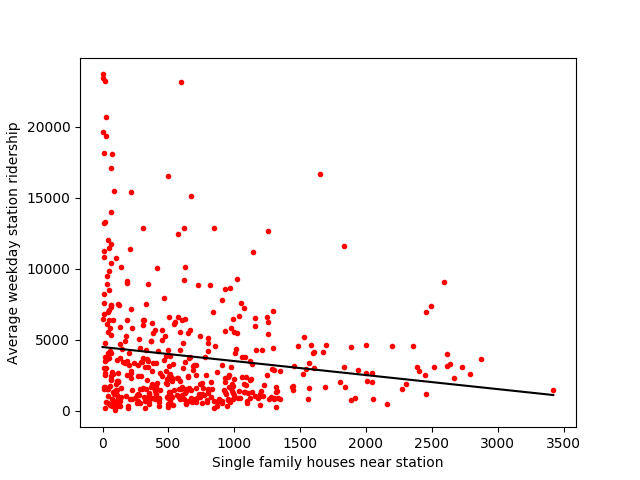
\includegraphics[clip,width=0.5\columnwidth]{exRegNegSlope}}
\caption{Single covariates against the response variable with ordinary least squares (OLS) line of best fit.}\label{fig:chartypes}
\end{figure}


In Yao \cite{Yao2007}, a distinction is made between `Need Index' features, a series of features that depend on the characteristics around the station and are independent of the transit network, and `Transit Network' features, which do depend on the travel time between stations of the transit network. To model network features for each station, the sum of each characteristic for every other station within 15 and 30 minutes transit time is included as a feature of the original station, as described in Section \ref{sec:net}. This provides us a quantitative way to express the 'centrality' dummy variable that is provided as a flag in many models \cite{Kuby2004, Durning2015}; centrality could be proportional to the count of population or jobs within 30 minutes of a station, for example. 

We translate zip code level data into transit station specific data by sampling each zip code's geographic area to determine proximity to a transit station. For each zip code near the transit network, a set of random points within that zip code is generated using rejection sampling. For each of the those points, one or more closest stations are determined. Each point is assigned to one or more station within walking distance, as defined in Section \ref{sec:walk}. Counts for the characteristics of each zip code, such as population or employment, are then assigned to each station proportional to the number of points assigned to each station.

\subsection{Definition of `Walking Distance'}\label{sec:walk}

The area within walking distance of a station is called its `catchment'. To generate a feature for a transit station, the total count of some characteristic within the catchment of that stations is considered. The standard transit catchment distance in literature for rail stations is one half mile (800 m). Guerra \cite{Guerra2012} suggests that one half mile is more appropriate for population as a feature while one quarter mile (400 m) is better for employment as a feature. A case study \cite{ElGeneidy2014} from a 2003 Montreal transit riders origin-destination survey concluded that approximately 50\% of riders of the city's urban rail transit walk less than 500 meters to their stations, while 90\% walk less than 1000 meters. The maximum walking distance is approximately 1500 meters. In another analysis, \cite{Gutierrez2011} found the optimal distance for  for assigning population and employment to a station was between 600 and 900 meters in straight line distance.

A significant concern when tabulating catchments is that in many of the densest regions of cities, there are many stations within a few hundred meters of each other. For example, from the Massachusetts State House in downtown Boston, there are seven urban rail stations on four different train lines within a 10 minute walk, according to Google Maps. Any of those stations could be the `best' place to board and disembark the train for a commute to work at the State House, depending on the direction and train line by which the commuter was arriving in downtown. It is important that we allow some `overlap' in catchment areas; people at one geographic location could use more than one station for various transit needs. 

Given this information, we choose cutoffs of 500 meters and 1000 meters for calculating station distances. For any location that has residents, jobs, or other desired countable characteristics, all stations within 500 meters will be considered equally likely to capture a share of that resident or job's transit demand. If there are no stations within 500 meters; then all stations within 1000 meters will be considered. 

\subsection{Rejection Sampling of Zip Code Shapefiles}\label{sec:sampling}

INCORPORATE NOTE HERE????

We translate zip code level data into transit station specific data by using a Monte Carlo method to estimate feature counts near transit stations. Sample points are generated within each zip code near the transit network. Those points are assigned to whichever stations are within walking distance of the station. The ratio of points assigned to each station to total points generated for each zip code is used to assign feature counts to each station. An algorithm for rejection sampling a single zipcode is provided in Algorithm \ref{alg:rejsamp}.


\begin{algorithm}\begingroup\fontsize{10}{10}\selectfont
\begin{algorithmic}
\State{ Given $zipcode$ is a single zipcode near the transit network }
\State{ Let $zipcode.latrange$ and $zipcode.lonrange$ be maximum and minimum latitude or longitude for $zipcode$ shapefile}
\State{ $n \gets$ max($zipcode.area$ in hectares, 1000)}
\State{ $randomPoints \gets \{\}$}
\While{ len($randompoints$) $< n$}\Comment{Generate $n$ random points within $zipcode$}
	\State{ $lon \gets $ random number $\in zipcode.lonrage$; $lat \gets $ random number $\in zipcode.latrage$}
	\State {$point \gets (lat, lon)$}
	\If { $point$ is inside $zipcode$ shapefile and $point$ is not inside exclusion areas}
		\State{ $randomPoints \gets point$}
	\EndIf
\EndWhile
\For{ $point \in randomPoints$}\Comment{Assignment of points to stations}
	\State{ $n_{0.5} \gets$ number of stations within 0.5 km of $point$}
	\State{ $n_1 \gets$ number of stations within 1 km of $point$}
	\If{ $n_{0.5} > 0$}
		\For{ $station$ within 0.5 km of $point$}
			\State{ $station$.characteristicValue $ += $ $zipcode$.characteristicValue}
		\EndFor
	\ElsIf {$n_1 > 0$}
		\For{ $station$ within 1 km of $point$}
			\State{ $station$.characteristicValue $ += $ $zipcode$.characteristicValue}	
		\EndFor
	\EndIf
\EndFor
\end{algorithmic}\endgroup\caption{Algorithm for estimating characeristic counts that are near transit stations}\label{alg:rejsamp}
\end{algorithm}



The US Census Bureau provides TIGER/Line shapefiles of each zip code tabulation area (ZCTA) in the United States at \url{https://www.census.gov/geo/maps-data/data/tiger-line.html}. Random points are generated in a rectangular box drawn around the extremities of each zipcode's shape; these random points are accepted if they are within the shapefile or rejected if they are outside it. Those points that are inside the shapefile are tested against author-created exclusion zones. These zones are shapes within the zip code's shapefile area that are known to not have any population, employment, or other countable characteristics. The exclusion zones are mostly drawn over water areas or large parks. Those points that are inside the exclusion zones are also rejected. This creates a set of points randomly drawn from the zip code's land area, not counting unoccupied regions like parks. 

The set of points is tested for their distance to any transit stations to determine which station catchments they fall in, as described in Section \ref{sec:walk}. The characteristic counts associated with each tested point are divided between all stations within 500 meters. If there are no stations within 500 meters, then the point is divided between all stations within 1000 meters. If no stations are within 1000 meters, that point is not assigned to any station. The total sum of points and fractional points assigned to each station is divided by the total points available to get the fraction of each of the zip code's characteristic data counts is assigned to that transit station. 

\begin{figure}
\begin{center}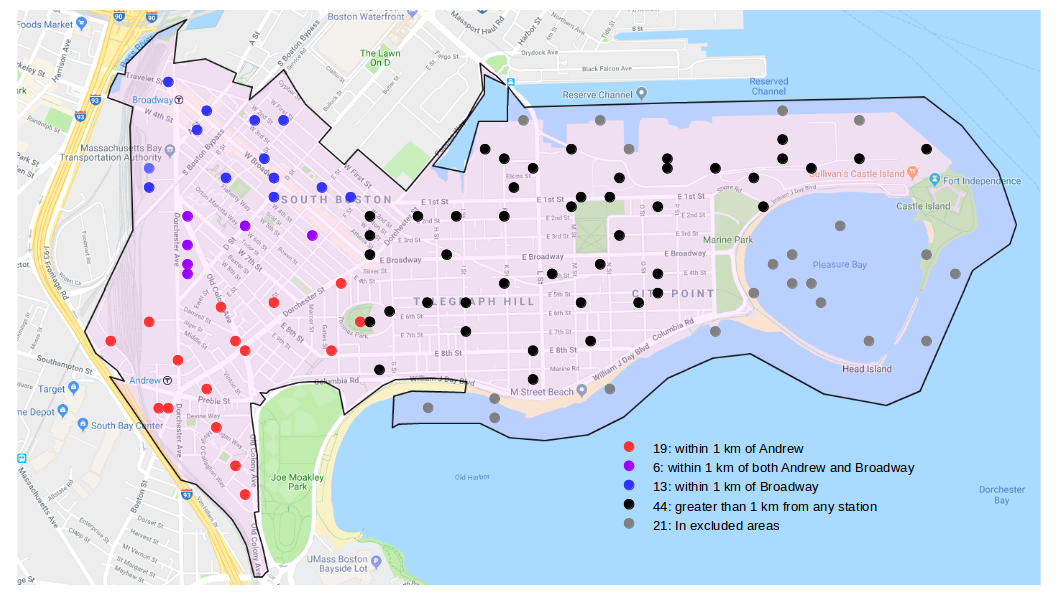
\includegraphics[scale=0.55]{geo_point_demonstration}\end{center}\caption{Illustration of nearest zip code estimation for zip code 02127.}\label{fig:f1}
\end{figure}


An example using zip code 02127, the South Boston neighborhood of Boston, illustrates the sampling method (Figure \ref{fig:f1}). 100 random points are selected within the area of the shapefile. Of these, 21 points indicated in gray are rejected due to exclusion areas based on water area, parks and abandoned port facilities. Of the remaining 79 points, 8 are within 500 meters of Andrew station, while 6 are within 500 meters of Broadway station. Moving out to the 1000 meter radius, 11 are within 1 km of Andrew station, for a total of 19 closest to Andrew; 7 are within 1 km of Broadway station for a total of 13 closest to Broadway; and 6 are within 1 km of both. The 6 stations within 1 km of both stations are divided evenly between the two. The total population of South Boston is 36494. Therefore, 
\begin{align*}
\text{Counts assigned to station} &= \frac{\text{\# points for one station} \cdot \sum\frac{\text{\# points for multiple stations}}{\text{\# stations for each point}}}{\text{\# points for zipcode}}\cdot\text{characteristic counts}  \\
&= \frac{19 + \frac{6}{2}}{79}\cdot 36494 \text{ people} \\
&= 10163 \text{ people}
\end{align*}
are assigned to Andrew station. Similarly, 7391 people are assigned to Broadway station. Summed over all zip codes near Andrew and Broadway stations, this shows how the total population within walking distance of the station is estimated. This calculation is performed for all countable features and all zip codes and summed total counts for each characteristic are used as a feature for each transit station. 

\subsection{Variance of Monte Carlo estimates}

With any Monte Carlo method for estimation, there is variance in the estimates generated. In this case, the variance will come primarily from the random locations of the points. It is possible that in different Monte Carlo trials, a station may get significantly more or less points nearby it. This is especially significant in areas of high population density; one extra or missing point could be worth hundreds or thousands of jobs in the densest areas of downtown Chicago or Boston. To keep variance to an acceptably low level, we must generate enough sample points that variation between trials is minimal. 

The land area of the zip codes near the studied transit networks vary in size from as small as 30 hectare in downtown Chicago to as much as 18100 hectares at the suburban end of transit lines in Dallas. To provide an appropriate balance between accuracy and processing speed, we use one random point per hectare, but with a minimum limit of 1000 points per zip code. This effectively provides over 10 points per hectare in for the zip codes in the densest parts of the studied networks: the downtown areas of Chicago and Boston. These areas also have the densest network of transit stations, with many stations within a kilometer of each other. In these denser areas, it is important to have enough points that the division of points between stations does not result in too much variance. 

We generate 100 sets of estimates for the a single feature (total population) for all stations in the six transit networks. Figure \ref{fig:mcvar}(a) shows a graph of means of total population estimates against standard deviation of the population estimates, while Figure \ref{fig:mcvar}(b) is means against coefficient of variation. The standard deviation shows an increasing linear relationship with the population mean. The coefficient of variation is never greater than 10.4\% and generally decreases with increasing estimated mean population. The mean coefficient of variance over all studied stations is 5.3\%. 

\begin{figure}[H]
\centering
\subfloat[Standard deviation versus mean by transit station]{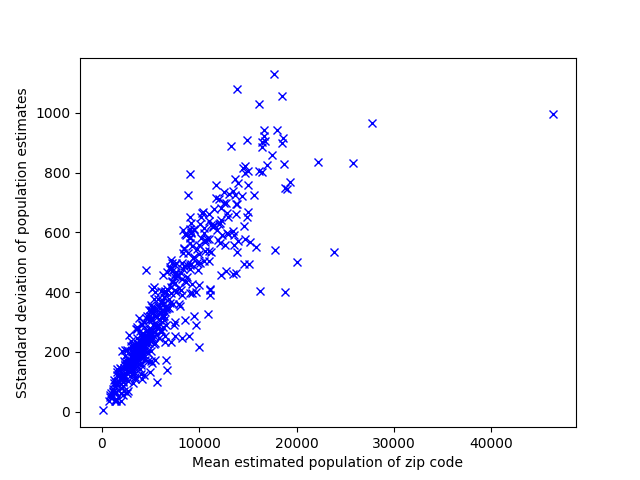
\includegraphics[clip,width=0.5\columnwidth]{estvarstdev}}
\subfloat[Coefficient of variation versus mean by transit station]{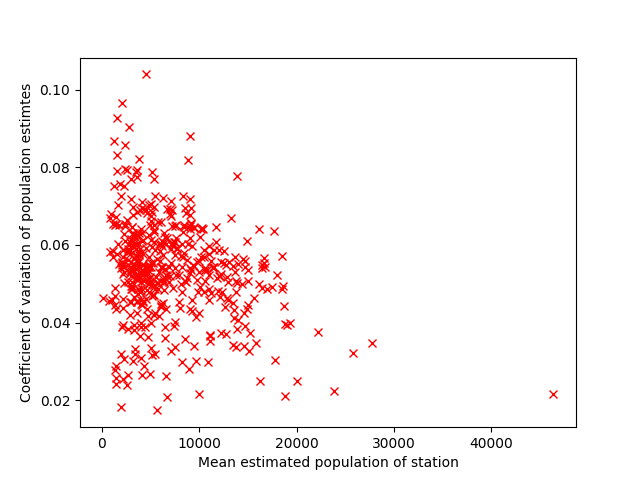
\includegraphics[clip,width=0.5\columnwidth]{estvarcov}}
\caption{Indications of variance for Monte Carlo estimates of the population feature}\label{fig:mcvar}
\end{figure}

IN CONCLUSION A RELATIVE ACCURACY OF +- 10%

\subsection{Generation of network-dependent features}\label{sec:net}

For each `Need Index' type feature generated by rejection sampling, a set of corresponding network-based features are generated to represent the sum total of a certain characteristic (such as population or employment) within a given travel time of that station. An algorithm for calculating network characteristics is shown in Algorithm \ref{alg:network}. 

\begin{algorithm}
\begin{algorithmic}
\For{$station \in$ transit network}
	\State$nearby15 \gets$ all other stations within 15 minutes travel time of $station$
	\State$nearby30 \gets$ all other stations within 30 minutes travel time of $station$
	\For{every characteristic in the model}
		\For{$otherStation \in nearby15$}
			\State{$station$.characteristicValue15 $+= otherStation$.characteristicValue}
		\EndFor
		\For{$otherStation \in nearby30$}
			\State{$station$.characteristicValue30 $+= otherStation$.characteristicValue}
		\EndFor
	\EndFor
\EndFor
\end{algorithmic}\caption{Algorithm for calculating network characteristic counts}\label{alg:network}
\end{algorithm}

The transit network is laid out as a directed graph, where nodes represent the transit stations and edges are weighted by the travel time between the stations. Travel times between stations are available in the transit schedules published by the appropriate transit agencies. Travel times can be different in different directions, following the published schedules. At transfer points, there is a separate node for a single station on each line. The multiple nodes for the same station have edges between them weighted by the average wait time between trains. The wait time is estimated at half the time between trains at the station being transferred to. For example, if one train arrives every 10 minutes, then a transfer to a node on that line at any station will have an estimated travel time of 5 minutes. Many transit agencies align arrival times so that one line will depart a few minutes after another train arrives. No attempt is made to capture this more complicated arrangement of estimated transfer times. 

\begin{figure}
\begin{center}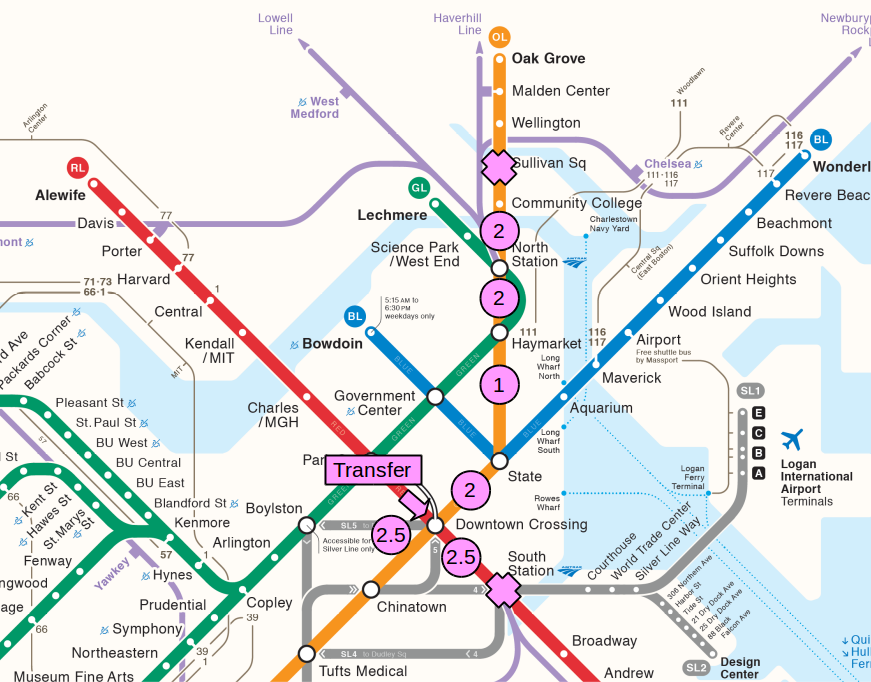
\includegraphics[scale=0.7]{transfer_demonstration}\end{center}\caption{Illustration of travel time calculation for Sullivan Square to South Station, in Boston.}\label{fig:f2}
\end{figure}

An illustration of the calculation of travel time between Sullivan Square and South Station in Boston is provided in Figure \ref{fig:f2}. Starting at Sullivan Square on the Orange Line southbound, there are four edge traversals totaling seven minutes to get to Downtown Crossing. From there, there is a 2.5 minute wait until a Red Line (also Southbound) train arrives, and 2.5 more minutes of travel to South Station. The total travel time is thus twelve minutes. 

For each station A and for the set of all stations (S) within 15 minutes of A; the counts of each `Need Index' type feature is summed over all stations of S. This is the count used for the corresponding network type feature of A. The same procedure is repeated for all stations within 30 minutes of A. Thus, for each `Need Index' type feature associated with a station in the feature set, there are two additional features: one summing the counts of that feature within 15 minutes and one within 30 minutes. 

These features are important for providing a measure of centrality to the network. Stations near the center of the network and at transfer points between lines will have higher counts of network features than peripheral stations. The other important function of the network features is to provide estimates of the total scale of system ridership. The more people, jobs, and other characteristics near transit stations, the higher the overall system ridership is expected to be. This is a key component of the model's portability between different city's transit networks. 




\subsection{Analysis of zip code characteristics by city}
\vspace{-15pt}
\begin{figure}
\centering
\subfloat[Boston - Blue; Chicago - Red; Los Angeles - Green]
{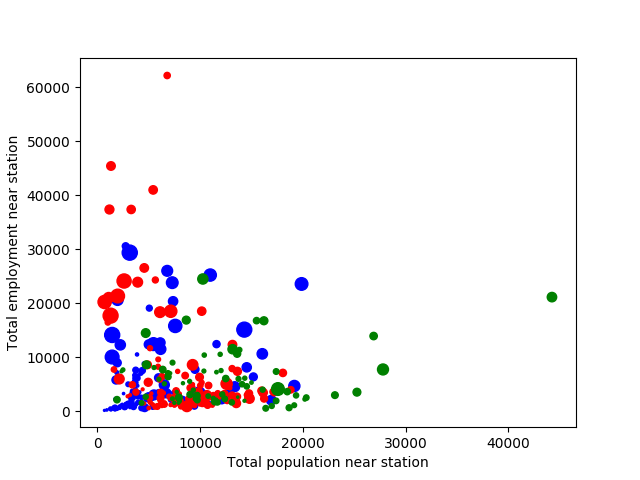
\includegraphics[clip,width=0.8\columnwidth]{localvars_large}}

\vspace{-15pt}
\subfloat[Atlanta - Blue; Dallas - Red; Denver - Green]{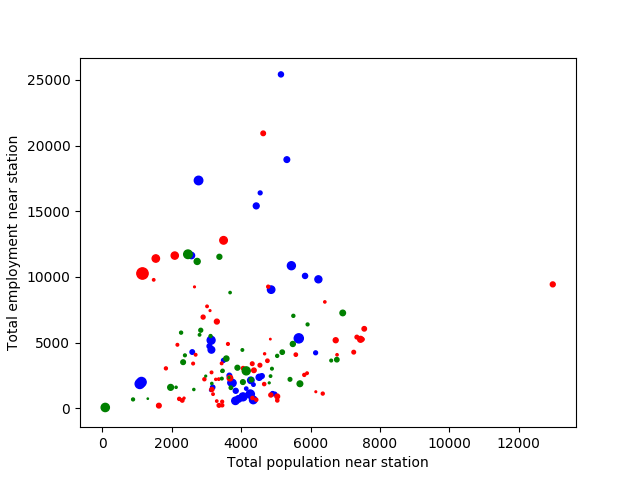
\includegraphics[clip,width=0.8\columnwidth]{localvars_small}}
\captionsetup{singlelinecheck=off, justification=centering}
\caption[]{Employment against population with a 15 minute transit ride for sets of three transit networks.\linebreak
Area of marker represents ridership of the station}\label{fig:localvars}
\end{figure}

The purpose of including multiple transit networks with varying levels of ridership is to ensure that the model captures a broad range of relationships between employment, population and other zip code characteristics on the one hand, and transit ridership on the other. Figure \ref{fig:localvars} shows the employment and ridership counts within walking distance assigned to each station on the transit networks. The ridership of each stations is proportional to the area of the marker for each station. We can see that there is a wide range of population and employment figures near transit stations. In our selection of six transit networks, some networks have much higher peaks of certain zip code characteristics than others, so the graphic is divided into two subfigures, one for the higher ridership networks and one for the lower. 

Station remoteness has a significant impact on the characteristics of stations. For example, the five highest population transit stations are all in Los Angeles. It is not true that the densest areas of Los Angeles have a higher population density than Boston or Chicago. Rather, the Los Angeles transit network has lower station density than Boston or Chicago in the areas of highest population density. Therefore, some stations in high population density areas of Los Angeles will have a transit catchment of up to two square kilometers. For Boston or Chicago, with closer station spacing and multiple lines, any point in the areas of highest population density will have four or more stations within walking distance.  

\begin{table}
\centering\begingroup\fontsize{10}{10}\selectfont
\begin{tabular}{l|cccc}
\toprule Network City&Total Population&Total Employment&Network length (km)&Avg Weekday Ridership \\ 
\midrule Chicago&1189454&872206&157&608472\\
Boston&622484&656375&98&591823\\
Los Angeles&935041&436846&169&254183\\
Atlanta&150171&207601&77&150237\\
Dallas&255092&261813&150&96069\\
Denver&161542&170631&149&75128\\
\bottomrule
\end{tabular}\endgroup
\caption{Network wide characteristics for the six transit networks considered in this thesis}\label{tab:netsize}
\end{table}

The overall characteristics of each transit network are found in Table \ref{tab:netsize}. There is a positive linear relationship between both population and employment and ridership at the network-wide level. However, the effect of network length is also significant. For example, Atlanta's population and employment near its transit stations are both lower than that of Dallas, but Atlanta's ridership is fifty percent larger. Atlanta's network length is about half that of Dallas, suggesting that Atlanta's transit accessible population and employment are compressed into a much smaller area. This density appears to be a significant factor in Atlanta's higher ridership. However, looking at Figure \ref{fig:localvars}(b), where Atlanta's stations are in the blue and Dallas' in red, it is not clear that Atlanta's stations have any individual advantage in population and employment. 

This shows the necessity of the network-dependent features. In Figure \ref{fig:networkvars}, we see the sum of population and employment within a 15 minute transit rider of each station, instead of within walking distance of each station. In Figure \ref{fig:networkvars}(b) we see that Atlanta's smaller network and more tightly spaced stations means that stations generally have more other stations within a given travel distance. Therefore, many of Atlanta's stations have higher network population and employment counts than their corresponding stations in Dallas. The inclusion of the network features will allow the regression model to more accurately predict the higher ridership for stations in Atlanta. 


\begin{figure}
\centering
\subfloat[Boston - Blue; Chicago - Red; Los Angeles - Green]
{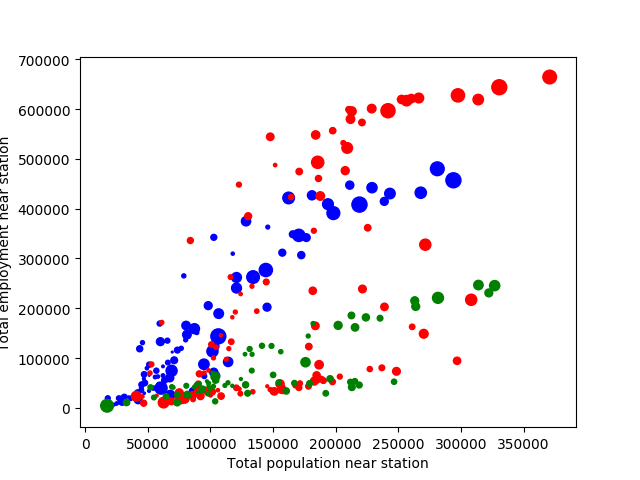
\includegraphics[clip,width=0.8\columnwidth]{networkvars_large}}

\vspace{-15pt}
\subfloat[Atlanta - Blue; Dallas - Red; Denver - Green]{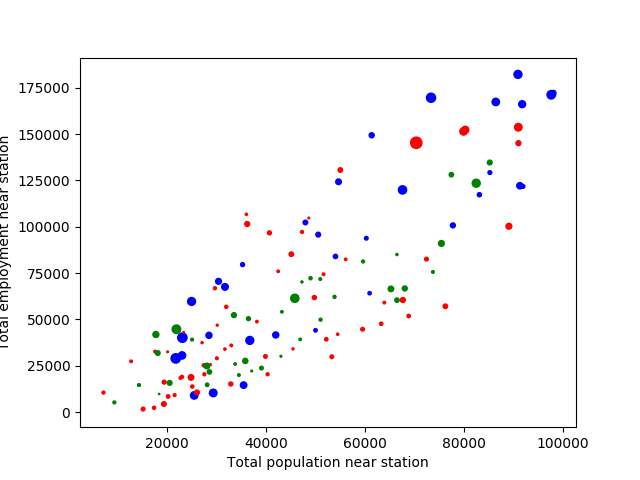
\includegraphics[clip,width=0.8\columnwidth]{networkvars_small}}
\captionsetup{singlelinecheck=off, justification=centering}
\caption[]{Employment against population with walking distance for sets of three transit networks.\linebreak
Area of marker represents ridership of the station.}\label{fig:networkvars}
\end{figure}




\section{Model generation and Error Metrics}

\subsection{Metrics for assessing accuracy of predictions}\label{sec:metric}

In general, the projected ridership forecasts of new transit infrastructure investments significantly overestimates transit ridership. The pioneering study in this field by Pickrell in 1989 \cite{Pickrell1989} found that for ten rail projects completed between 1977 and 1985, and assessed between 1986 and 1989, the actual ridership was between 28\% and 85\% lower than projected. A 2006 study \cite{Flyvbjerg2006} of 25 major passenger rail projects in 14 nations found that 21 of the projects had actual ridership below projections, with the average true system ridership 48\% below the projection. Accurate assessment of projection accuracy is imperative for creating ridership estimates that serve the public interest.

To assess the predictions from regression analysis, there should be two metrics used: one for the total system ridership, and another for station level ridership. Following Pickrell, the metric for system-wide projection accuracy is standard percentage error in total system ridership, which we will refer to as system error. This error is
$$E_{system} = \dfrac{\left|\,\sum\limits_{i\,\in\,\text{stations}} y_{i, proj} - \sum\limits_{i\,\in\,\text{stations}} y_{i, true}\,\right|}{\sum\limits_{i\,\in\,\text{stations}} y_{i, true}},$$
where $y_{proj}$ is the projected ridership and $y_{true}$ the true ridership for each station, and each is summed over all stations.

Hardy \cite{Hardy2010} extends Pickrell's analysis by including absolute station error for stations on newly added sections of an existing transit network. Following Hardy, a measure of station level error on a network is the summed absolute error of all station projections. The rail networks in this study vary widely in total ridership; therefore, to allow network-to-network comparison, this summed absolute station error can divided by total system ridership. The resulting metric for station error given a projected ($y_{proj}$) and actual ridership ($y_{true}$) is 
$$E_{station} = \dfrac{\sum\limits_{i\,\in\,\text{stations}}\left|\,y_{i, proj} - y_{i, true}\,\right|}{\sum\limits_{i\,\in\,\text{stations}} y_{i, true}}.$$


INSERT DIVIDING LINE BETWEEN THE TWO FIGURES!!!

\begin{figure}
\centering
\begin{minipage}{0.45\textwidth}
\centering
\subfloat[Ridership against population. Linear regression in red, log regression in blue.]{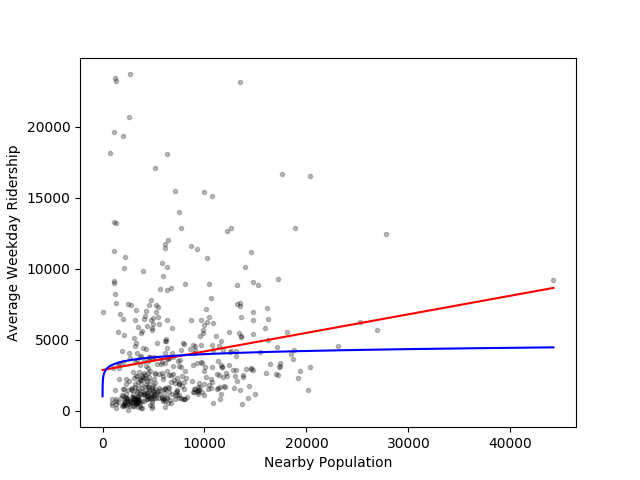
\includegraphics[clip,width=\columnwidth]{popvrider}}

\subfloat[Residual from linear regression against population]{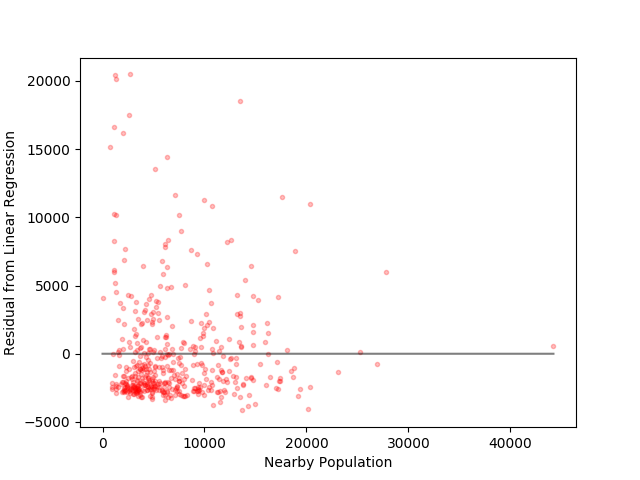
\includegraphics[clip,width=\columnwidth]{poplinresid}}

\subfloat[Residual from log regression against population]{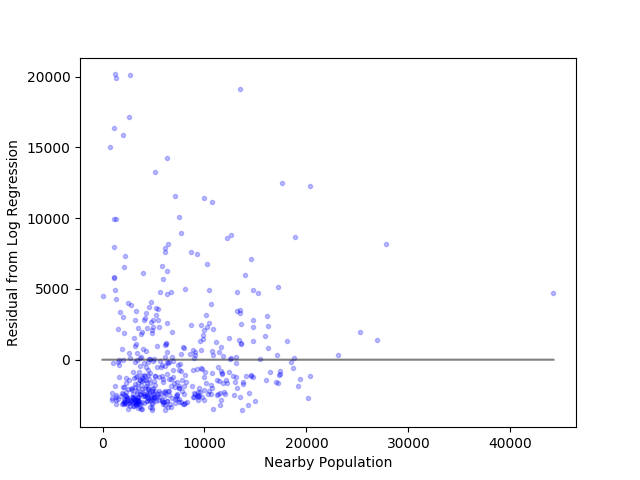
\includegraphics[clip,width=\columnwidth]{poplogresid}}
\caption{Analysis of population regression}\label{fig:popresid}
\end{minipage}\hfill
\hspace{5pt}
\unskip\vrule
\hspace{10pt}
\begin{minipage}{0.45\textwidth}
\centering
\subfloat[Ridership against employment. Linear regression in red, log regression in blue.]{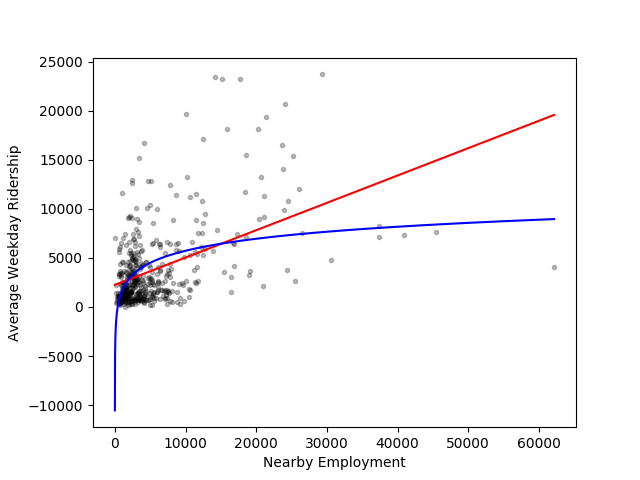
\includegraphics[clip,width=\columnwidth]{empvrider}}

\subfloat[Residual from linear regression against employment]{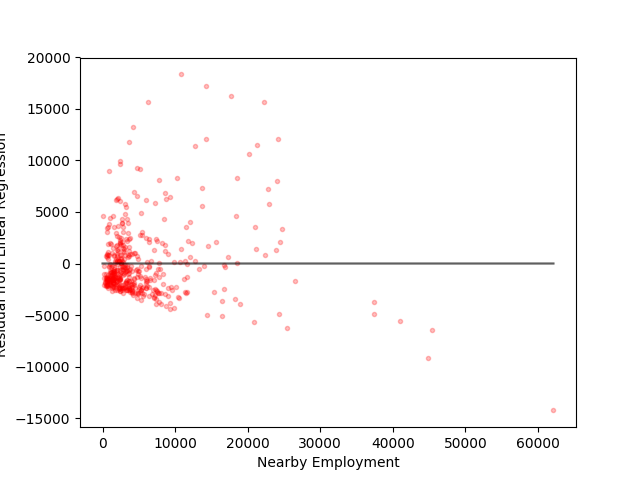
\includegraphics[clip,width=\columnwidth]{emplinresid}}

\subfloat[Residual from log regression against employment]{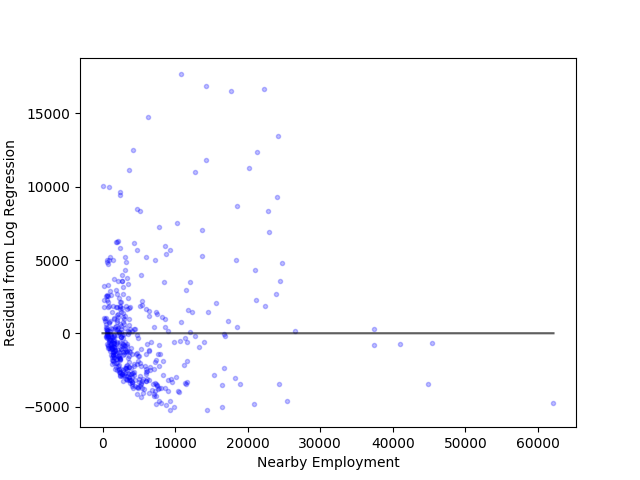
\includegraphics[clip,width=\columnwidth]{emplogresid}}
\caption{Analysis of employment regression}\label{fig:empresid}
\end{minipage}\hfill
\end{figure}


\subsection{Data distribution and regression selection}

Regression models for station level ridership have used ordinary least squares regression \cite{Kuby2004, Taylor2008, Currie2011, Durning2015, Gutierrez2011} to generate predictions. We investigate the applicability of more complex regression models, and whether or not these other regression types can provide better modeling accuracy.

The range of the dependent variable, average weekday ridership at a station, has range $[0, \infty)$. The log link function has this range and so it is reasonable to assume that there may be a logarithmic relationship between characteristics and ridership. To test the viability of the log link, we can compare a linear least squares line of best fit with a line of best fit using the logarithm of the ridership as the response variable. CHANGE THESE MODELS TO USE GLM WITH LOG LINK

There are generally two types of feature included in this survey: those that are related to population and those that are related to employment. A plot of all stations' population versus ridership appears in Figure \ref{fig:popresid} with linear and logarithmic regression lines and residuals. A similar treatment for employment versus ridership appears in Figure \ref{fig:empresid}. In Figures  \ref{fig:popresid}(a) and \ref{fig:empresid}(a), a linear and logarithmic best fit line, derived as shown in Section \ref{sec:ols} below, are fitted to the data. The residuals from the linear regression line are plotted in (b) and from the logarithmic regression in (c) of each figure. 

The coefficient of determination for the two regression types for both population and employment are shown in Table \ref{tab:regr2}. Judging from the coefficients of determinations and the distributions of the residuals, there does not appear to be any clear modeling advantage from using either an identity or logarithmic link function. 

\begin{table}[H]
\centering
\begin{tabular}{lcc}
\toprule Variable&Linear R$^2$&Log R$^2$ \\ 
\midrule Population&0.0267&0.0034 \\
Employment&0.1948&0.1878 \\
\bottomrule
\end{tabular}
\caption{Regression of Population and Employment against ridership}\label{tab:regr2}
\end{table}


The metrics for projection accuracy introduced in Section \ref{sec:metric} depend on the absolute difference between actual and predicted ridership. This suggests that regression using the Least Absolute Deviation (LAD) (ADD SECTION DEFINING LAD!!!!) loss function is appropriate for this problem. Since the response variable (ridership) has a value of integer counts, and the variance of ridership increases with increasing employment, we will also investigate the use of a Poisson model. Finally, we will use ordinary least squares (OLS) regression as a baseline comparison, to see if the other methods have any performance advantage compared to the currently used regression type. Since we are not certain whether a log or linear link function is most appropriate, we will test the Poisson and least squares regression with both log and linear link functions.

There are 94 possible features, while some transit networks have as few as 38 stations. Feature selection is necessary to prevent the model from being overspecified. We use two methods of feature selection for each of the five regression types: LASSO regression described in Section \ref{sec:lasso} and a stepwise forward selection method described in Section \ref{sec:fs}. 

Upon performing any regression analysis, it becomes immediately apparent that one set of features is different from the others. Estimating station ridership using only the number of students within a 15 or 30 minute transit trip of each station provides a very accurate measurement of system level ridership. These variables are represented in the model as \texttt{15net\_students} and \texttt{30net\_students}, respectively. We show the results of a single variable OLS regression of the one variable against ridership. The scores are the average of the six way cross-validation across the six transit networks in the study; each of the six networks is used as the test set in one case, while the other five transit networks are used as the training set. The `best' scoring other feature (\texttt{15net\_hunits\_old}; the number of housing units built before 1940 within a 15 minute transit ride) is shown for comparison.

\begin{table}[H]
\centering
\begin{tabular}{lcc}
\toprule Variable&System Error&Station Error\\
\midrule 30net\_students&0.1016&0.5961\\
15net\_students&0.0946&0.6197\\
15net\_hunits\_old&0.2854&0.6700\\ 
\end{tabular}
\caption{Error for single variable OLS for selected features}\label{tab:students}
\end{table}

The system error scores for \texttt{30net\_students} and \texttt{15net\_students} are much lower than for any other variable, while the station error for these features are also lower than any other features. As we will see, the single-feature OLS of either of these features produces a model that is approximately as good as any other model we will develop. This raises questions about the relationship between this feature and the response variable. It is possible that the population of students within walking distance of a transit station is driven by the availability of local transit, and not the other way around; that is, students particularly among a larger population will chose their housing locations based on availability of transit. In that case, the number of students is not a valid explanatory variable. Since the relationship is unclear and the features are outliers, we will remove all features derived from number of students from the model.



\subsection{Derivation of Regression methods}
For the five regression types described, the methodolody and packages used are described below. A chart of packages used for implementation is presented in Table \ref{tab:regtype}.

\begin{table} [H]
\centering
\begin{tabular}{lll}
\toprule Regression&Link&package\\
\midrule Least Squares&Identity&LASSO: \texttt{glmnet} for Python\\
&&Forward Selection: \texttt{statsmodels} for Python\\
&Log&LASSO: Author-created\\
&&Forward Selection: \texttt{statsmodels} for Python\\
LAD&Identity&LASSO: \texttt{flare} for R\\
&&Forward Selection: \texttt{statsmodels} for Python\\
Poisson&Log&LASSO: \texttt{glmnet} for Python\\
&&Forward Selection: \texttt{statsmodels} for Python\\
&Identity&LASSO: Author-created\\
&&Forward Selection: \texttt{statsmodels} for Python\\
\bottomrule
\end{tabular}
\caption{Regression types and packages used in analysis.}
\label{tab:regtype}
\end{table}



\subsubsection{Least squares regression}\label{sec:ols}

Ordinary Least Squares (OLS) regression is a model,
\[Y = \theta X + \epsilon\] where $\theta$ is a parameterization and $\epsilon$ is assumed to be normally distributed. The expected value of any element of $Y$ is the corresponding element of $\theta X$:
\[E(Y\,|\,X; \theta) = \theta X\]
Here, $Y$ is length $m$ a vector of response variables; $\theta$ is a length $p$ vector of parameters and $X$ is an $m\times p$ matrix of covariates. The sum of squared residual measure of model fit gives us an objective function to minimize for a solution
\[\hat{\theta} = \argmin_{\theta\in\mathbb{R}^p}\sum_{i=1}^m \left(y_i - \theta x_i\right)^2.\]

For LASSO regression, an additional constraint on the parameters is introduced where 
\[\sum_{j=1}^p |\theta_j|\leq t.\] We apply this constraint to OLS to solve for parameters such that
\[\hat{\theta} = \argmin_{\theta\in\mathbb{R}^p} \frac{1}{N}\sum_{i=1}^m \left(y_i - x_i^\top\theta\right)^2 + \sum_{j=1}^p\lambda_j\theta_j.\]
The tuning parameter $\lambda$ is proportional to the strength of the regularization penalty. The larger the $\lambda$, the fewer features will be selected. The LASSO solver used for both Least Squares and Poisson in this experiment is the \texttt{glmnet} package \cite{glmnet}; in this package, the optimal $\lambda$ is identified by using a grid search and cyclical coordinate descent.  

For least squares regression with a log link, or loglinear regression, we transform all entries in the $y$ vector of response variables by the natural logarithm so that 
$$\log{y} = \theta X + \epsilon.$$
With this transformation of the response variable, we perform a regular or LASSO regression as above. We then use the exponential function of predicted station level ridership so that the range of the predictions is in the same units across all regression types.

\subsubsection{Poisson regression with Log link}

Poisson regression is performed with its canonical log link. The mean of the predicted Poisson distribution is given by 
\[E(Y\,|\,X;\theta) = e^{\theta X}.\]
The Poisson probability mass distribution becomes
\[p(y_1, ..., y_m|x_1, ..., x_m; \theta) = \prod_{i=1}^m \frac{e^{y_i\theta x_i}e^{-e^{\theta x_i}}}{y_i!}\]
with a negative log-likelihood expression
\[-\mathcal{L}(\theta|X, Y) = \sum_{i=1}^m e^{\theta x_i}-y_i\theta x_i \]
ignoring the constant factorial term which falls out in differentiation. This convex function is the objective function and is minimized over $\theta\in\mathbb{R}^p$.

For LASSO regression, we minimize the parameters \cite{Young2007} over  
\[\hat{\theta}(\lambda) = \argmin_{\theta\in\mathbb{R}^p}  \frac{1}{N}\sum_{i=1}^m e^{\theta x_i}-y_i\theta x_i  + \sum_{j=1}^p\lambda_j\theta_j.\]


\subsubsection{Poisson regression with Identity link} \label{sec:poisI}

With no suitable package to perform LASSO regression using Poisson regression and the identity link, we implement this method using Python.

For the identity link, the mean of the predicted Poisson distribution is given by $$E(Y\,|\,X;\theta) = \theta X$$ where $Y$ is length $m$ a vector of response variables; $\theta$ is a length $p$ vector of parameters and $X$ is an $m\times p$ matrix of covariates. This mean is entered into the Poisson probability mass distribution to get 
$$p(y_1,...,y_m|x_1,...,x_m;\theta) = \prod_{i=1}^m \frac{\left(\theta x_i\right)^{y_i}e^{-\theta x_i}}{y_i!} $$
The negative log likelihood of this distribution is the objective function
$$-\mathcal{L}\left(\theta\,|\,X, Y\right) = \sum_{i=1}^m -y_i\log{\left(\theta x_i\right)} +\theta x_i. $$ This function is convex and so the minimum can be obtained using convex optimization methods. 

To implement LASSO \cite{Tibshirani1996}, we use the primal-dual interior point method from Boyd and Vandenberghe \cite{Boyd2004}. There are no equality constraints for this problem, and only one inequality constraint.

\begin{center}\begin{tabular}{ll}
minimize &$f_0(x)$\\
subject to &$f_i(x) \leq 0, \quad i = 1, ..., m$.
\end{tabular}\end{center}


 Both $f_0$ and $f_1$ must be convex and twice continuously differentiable. But in LASSO the constraint is $||\boldsymbol{\theta}|| < t$, which is a function of the absolute value of $\theta_i$; a non-differentiable function. Therefore, we define the constraints as 


\begin{align}
f_0(\theta) =& \sum_{i=1}^m -y_i\log{\left(\theta x_i\right)} +\theta x_i
&\nabla f_0(\theta) = \sum_{i=1}^m \dfrac{x_i\left(y_i-\theta x_i\right)}{\theta x_i}\quad
&\nabla^2 f_0(\theta) = \sum_{i=1}^m\dfrac{y_i x_i^2}{\left(\theta x_i\right)^2}\label{eq:objective}\\[0.2in]
f_1(\theta) =& \sum_{j=1}^p\,-\theta_j
&\nabla f_1(\theta) = \sum_{j=1}^p -1 = -p\quad
&\nabla^2 f_1(\theta) = 0\label{eq:constraints}
\end{align}
We establish the modified Karush-Kuhn-Tucker (KKT) equations for solving this problem using a Newton method. The objective function to be minimzed is $f_0$ and the inequality constraint is $f_1$. There is no equality constraint, which takes the form $Ax = b$ in the usual KKT conditions; therefore these terms are not present in our equations. Given that there are $p$ features and $m$ data points in our problem, then $f_0, f_1, f_2: \mathbb{R}^p \rightarrow \mathbb{R}.$ 

The Newton steps for solving the modified KKT equations are given by 

\[r_\gamma(\theta, \lambda) = \begin{bmatrix}
\nabla f_0(\theta) + \lambdaup\nabla f_1(\theta)\\
-\text{diag}(\lambdaup)f_1(\theta) - \frac{1}{\gamma}\mathbb{I}
\end{bmatrix} = \begin{bmatrix}
r_{dual}\\r_{cent}
\end{bmatrix}\,.\]
With the values for the constraint function ($f_1$) and its derivatives from (\ref{eq:constraints}), we define  $r_{dual}$ and $r_{cent}$ as 
\begin{align}
r_{dual}&= \nabla f_0(\theta) - \lambda\label{eq:rdual}\\
r_{cent}&= \text{diag}(\lambdaup)\theta - \frac{1}{\gamma}\mathbb{I}
\end{align}
For a current point $y = \left(\theta, \lambdaup\right)$, the next Newton step will be $\Delta y = \left(\Delta\theta, \Delta\lambdaup\right)$. The Newton step is characterized by the linear equation
\[r_\gamma(y + \Delta y) \approx r_t(y) + \nabla r_t(y)\Delta y = 0\] or 
\[\begin{bmatrix}
\nabla^2f_0(\theta) + \lambdaup\nabla^2f_1(\theta)&\nabla f_1(\theta)\\
-\text{diag}(\lambdaup)\nabla f_1(\theta)&-\text{diag}\left(f_1(\theta)\right)
\end{bmatrix}\begin{bmatrix}
\Delta\theta \\ \Delta\lambdaup
\end{bmatrix} = - \begin{bmatrix}
r_{dual}\\r_{cent}
\end{bmatrix}.\]
We retain the objective function $f_0$ and its gradient and Hessian as defined in (\ref{eq:objective}) but we plug in values for the constraint function from (\ref{eq:constraints}) to get a set of two linear equations:
\begin{align}
\nabla^2f_0(\theta)\Delta\theta - \Delta\lambdaup &= -r_{dual}\label{eq:dualeq}\\
\text{diag}(\lambdaup)\Delta\theta + \text{diag}(\theta)\Delta\lambdaup &= -r_{cent}\,\label{eq:centeq}
\end{align}
We solve (\ref{eq:centeq}) for $\Delta\lambdaup$ in terms of $\Delta\theta$,
\begin{equation}
\Delta\lambdaup = \frac{-r_{cent} - \text{diag}(\lambdaup)\Delta\theta}{\theta}\, ,\label{eq:dellam}
\end{equation}

and plug into (\ref{eq:dualeq}) to get
\begin{align}
\nabla^2f_0(\theta)\Delta\theta +\frac{r_{cent}}{\theta} + \frac{\text{diag}(\lambdaup)\Delta\theta}{\theta} &= -r_{dual}\nonumber\\ 
\left(\nabla^2f_0(\theta) + \frac{\text{diag}(\lambdaup)}{\theta}\right)\Delta\theta &= -r_{dual} - \frac{r_{cent}}{\theta}\,.\label{eq:delbeta}
\end{align}
The value of $\Delta\theta$ is solved from the linear equation in (\ref{eq:delbeta}).

\begin{algorithm}\begingroup\fontsize{10}{10}\selectfont
\begin{algorithmic}
\State{ Given $\epsilon > 0$}
\State
\While {$||r_{dual}||_2 < \epsilon$ and $\eta \leq \epsilon$}
	\State $\gamma \gets p\mu/\eta$
	\State Compute $\Delta\theta$ and $\Delta\lambdaup$ using (\ref{eq:dellam}) and (\ref{eq:delbeta}).
	\State Determine step length $s>0$
	\State $\theta \gets \theta + s\Delta\theta$
	\State $\lambdaup \gets \lambdaup + s\Delta\lambdaup$
\EndWhile
\end{algorithmic}\endgroup\caption{Algorithm for solving interior point primal-dual problem}\label{alg:piip}
\end{algorithm} 

Minimization over $\theta$ and $\lambdaup$ is obtained by by iteration, as shown in Algorithm \ref{alg:piip}. The duality gap, the difference between the primal and dual solutions, is not necessarily feasible during each iteration of the interior point method. Therefore, a surrogate duality gap is $\eta(\theta, \lambdaup) = -f_1(\theta)^\top\lambda = \theta\lambda$. A constant scaling constant for $\gamma$ is $\mu$; $p$ is the number of features in the covariate matrix, or the length of $\theta$ and $\lambdaup$. During each iteration, we update $\Delta\theta$ in accordance with (\ref{eq:delbeta}) and $\Delta\lambdaup$ in accordance with (\ref{eq:dellam}). The iterations repeat until both the surrogate duality gap and the dual residual are below a certain threshold ($\epsilon$).

\vspace{50pt}



\begin{table}[H]
\begingroup\fontsize{8}{15}\selectfont
\centering
\begin{tabular}{ll|ccccc}
\toprule
Regression Type&Feat Select Type& Min System Err&Min Station Err& \# Features Selected& Avg System Err& Avg Station Err\\
\midrule
LstSq - Linear&Pop and Emp only&0.0451&0.5324&2&0.5172&0.8307\\
LstSq - Linear&Best Single Feat&0.0465&0.4731&1&0.2852&0.6700\\
\midrule
LstSq - Linear&Stepwise&0.0216&0.4461&12&0.1919&0.6197\\
LstSq - Log&Stepwise&0.0450&0.4997&16&0.1741&0.5789\\
Poisson - Log&Stepwise&0.0426&0.4861&15&0.2184&0.6218\\
Poisson - Identity&Stepwise&0.0009&0.4113&8&0.1936&0.6071\\
LAD&Stepwise&0.0005&0.3986&4&0.1792&0.5610\\
\midrule
LstSq - Linear&LASSO&0.0152&0.4717&9&0.3455&0.7057\\
LstSq - Log&LASSO&0.0404&0.4501&19&0.4041&0.6773\\
Poisson - Log&LASSO&0.0892&0.4753&10&0.4857&0.7731\\
Poisson - Identity&LASSO&0.0721&0.4516&10&0.4214&0.7142\\
LAD&LASSO&0.0235&0.5867&23&0.6263&0.8629\\
\end{tabular}
\caption{Results of regression analysis, compared with some baseline measures}\label{tab:rresults}
\endgroup
\end{table}


\subsection{Feature selection by LASSO regularization}\label{sec:lasso}

Least Absolute Shrinkage and Selection Operator (LASSO) regression can be used to perform feature selection for regression analysis. The LASSO method adds a regularization term to an objective function to penalize regression coefficients. By forcing the sum of the absolute values of all regression coefficients to be less than a fixed value, some regression coefficients are set to zero, thereby eliminating them from the model. 

TALK ABOUT SCALING????

PERHAPS ALL THIS TO THE INTRO ???


An important part of the LASSO solution is selection of $\lambdaup$, the penalty coefficient. OLS and Poisson LASSO regression are performed using the \texttt{glmnet} package in Python, which does automatic $\lambdaup$ selection through a grid search (MORE DETAILS HERE!!!!!!). LAD LASSO is performed using the \texttt{flare} package in R.  For \texttt{flare} the author created a $\lambdaup$ grid search algorithm comparable to that performed by \texttt{glmnet}. The Poisson LASSO with identity link is performed by author supplied code, where $\lambdaup$ is solved concurrently with the regression parameters ($\theta$) by an interior point solver, as detailed in section \ref{sec:poisI}.  

The various LASSO regression types have a large variance in number of features chosen, both between transit networks and between regression types, shown in Table \ref{tab:lassoFeatNum}. Since the six way cross validation produces a different set of selected features for each transit network, we must develop a means for determining a `best' feature set for a common comparison. To represent the results of the LASSO regression, all features that are selected by four or more of the six cross-validation trials are used. 

The LAD LASSO regression chooses an average of 48 features across the six-way cross validation. This is far too high: the transit networks have between 37 and 138 stations. In order to use a more reasonable feature set; we increase the selection requirement for LAD LASSO to only those features selected by five or more of the six cross-validation trials are used. The large number of features selected by LAD LASSO regression may result from any differences in the $\lambda$ selection method used by the computing packages. 

\begin{table}[H]
\begingroup\fontsize{10}{15}\selectfont
\centering
\begin{tabular}{l|cccccc}
Regression Type&Atlanta&Boston&Chicago&Dallas&Denver&Los Angeles\\
\midrule
LstSq - Linear&10&2&8&9&10&17\\
LstSq - Log&26&12&17&22&28&46\\
Poisson - Log&11&5&12&26&27&29\\
Poisson - Identity&12&15&13&12&11&12\\
LAD&36&52&48&54&47&53\\
\end{tabular}
\caption{Number of features selected by LASSO; by transit network and regression type}\label{tab:lassoFeatNum}
\endgroup
\end{table}

The LASSO solution optimizes station-type error. The loss function for each LASSO method is dependent on the regression type: Least Squares loss, Poisson loss, or Least Absolute Deviation loss. In each case, the loss is the sum of a function of the predicted value, $\theta x_i$, and true value $y_i$, for each station. In this, the loss for each of these regression types resembles a station-type error. A system type error would be a loss function that is a function of the the predicted values summed over all stations, $\sum_i \theta x_i$, and the true values summed over all station, $\sum_i y_i$.

The features selected by four of the six cross-validation trials (or five trials, in the case of LAD) are used as the basis for generating the overall metrics in Table \ref{tab:rresults}. For all regression types, the LASSO method of feature selection performs significantly worse than the forward selection method. Several of the LASSO selections have too many features, and some of the poor accuracy may be attributable to overfitting. The results in Table \ref{tab:rresults} allow a comparison of the LASSO regression against some baseline measures, such an Ordinary Least Squares regression using only population and employment within walking distance. The LASSO methods do not significantly outperform this very simple model.


\subsection{Feature selection by stepwise forward selection}\label{sec:fs}


Since the data set for this problem is small--with only 466 total stations--we can validate the LASSO results using a stepwise forward selection approach. This method is a greedy search of all possible features to find the best combination of features that minimizes our error metrics. Each regression method and link function are tested in this way. First, for all features, we perform a single covariate regression against the response variable, ridership. Each feature is evaluated in six-way cross validation, where each of the six transit networks is used as the test set once, while the other five are used for the training set during each cross validation trial.


MORE DETAILS ABOUT CRITERION FOR SELECTING A NEW FEATURES

From the results of the single covariate regression, we choose the feature that gives us the lowest error score. Since LASSO selected features based on optimization of station-type error, we select the one feature that predicts ridership with the lowest station error. System error is ignored in order to ensure that our selection metrics are as similar as possible to LASSO's selection metrics. After choosing a feature in the first step; in the second step we perform a two covariate regression against ridership. The feature selected in the first round is used, and we test all other features as the second covariate. The second feature that yields the lowest station error is then selected. The subsequent steps continue with multiple regression using all of the already chosen features. We select the fist 25 features with this method and graph the resulting system and station error scores in Figure \ref{fig:bfscores}. 

\begin{figure}
\centering
\subfloat[Station Error against number of variables selected]{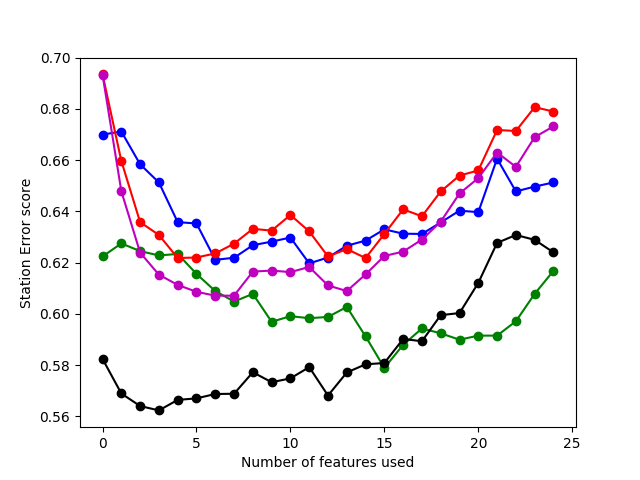
\includegraphics[clip,width=0.5\columnwidth]{fsstaerrs}}
\subfloat[System Error against number of variables seleted]{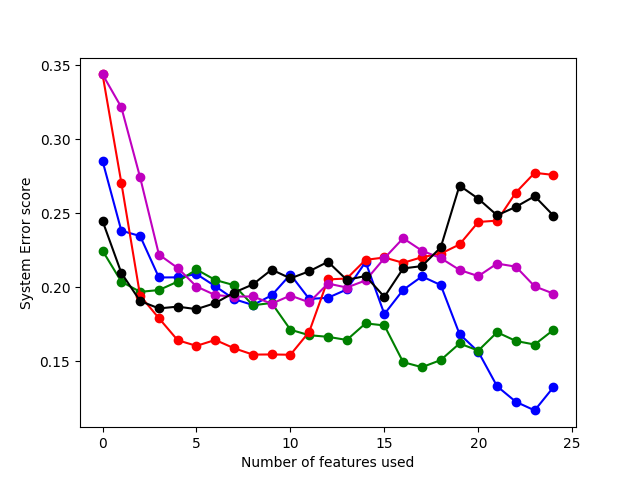
\includegraphics[clip,width=0.5\columnwidth]{fssyserrs}}
\captionsetup{singlelinecheck=off, font=scriptsize, justification=centering}
\caption[]{
Error against number of features used for stepwise forward selection\linebreak
Blue - Least Squares Linear; Green - Least Squares Log; Red - Poisson Log; Magenta - Poisson Identity; Black - LAD
%\begin{itemize}\setlength\itemsep{-5pt}
%\item Blue - Least Squares Linear
%\item Green - Least Squares Log
%\item Red - Poisson Log
%\item Magenta - Poisson Identity
%\item Black - Least Absolute Deviation
%\end{itemize}
}
\label{fig:bfscores}
\end{figure}

The error scores in Figure \ref{fig:bfscores} are averaged across the six-way cross validation. In general, each of the error scores decreases with the addition of new features up to a certain number of covariates, and then increases again. The minima for the system and station errors do not coincide with each other for any of the five regression methods, so there is a range of features which produce very similar error scores. In keeping with the optimization of LASSO on station-type loss functions, we will select as `best' the set of features that has the lowest station error. 

Our chosen metric of station error closely resembles the Least Absolute Deviation loss function. Therefore, it is not surprising that this regression type performs the best on the Station Error metric, having the lowest station error for up to 15 features. An interesting result of LAD regression is that the station error curve has its minimum much earlier than the other regression types, which show constant decreasing station error for at least the first six features. In the system error metric, the LAD regression loses its advantage. Instead, both the Least Squares regression methods produce low system error scores with increasing numbers of variables. 

The minimum scores from each regression type are recorded in Table \ref{tab:rresults} along with the average score over the range of good features. The stepwise regression significantly outperforms the LASSO regression in creating feature combinations that can accurately predict ridership in unknown transit networks. An OLS regression of the best single feature (the number of housing units built before 1940 within a 15 minute transit ride) is provided in Table \ref{tab:rresults}. All the stepwise regression methods outperform this baseline method. 

\subsection{Analysis of selected features}

A summary of selected features is given in Table \ref{tab:featuresum}. There are ten total regression methods used for feature selection; five LASSO methods and five forward selection methods. The count column in Table \ref{tab:featuresum} shows the number of times out of ten that each feature was selected. For example, the \texttt{near\_hospitality} feature was selected by all ten methods.

As seen in Table \ref{tab:rresults}, some of the regression types are better than others. Therefore, instead of simply counting whether or not a feature is selected by a regression type, we can weight its selection by the effectiveness of the each regression type. For the two error metrics, system and station error, the each regression method's score from Table \ref{tab:rresults} is transformed to the range $[0, 1]$, so the best performing regression type in each metric is weighted as 1, while the worst is rated at 0. (EXPLAIN THE WEIGHTING!!!!) For each feature, selection is weighted according to the regression type that selected it. These weighted selection counts are then rescaled to the range $[0, 10]$ and displayed in Table \ref{tab:featuresum} as the System Weighted and Station Weighted columns.

The weighted columns give insight into which features were selected by the best methods. Features with weighted scores greater than their count were only selected by the most accurate regression types; for example \texttt{near\_medical}, the number of medical jobs within walking distance, or \texttt{near\_hunits\_large}, the number of housing units in apartment buildings of 20 or more units. Other features with weighted scores less than their count were selected by the least accurate regression types. Examples here are \texttt{15net\_hunits\_attached}, the number of townhomes and 2-4 unit apartments within a 15 minute transit ride, and \texttt{15net\_hospitality}, the number of restaurant and hotel jobs within a 15 minute transit ride. 

The highly rated features display a mixture of potential correlation and causation with respect to transit ridership. For example, a major university is likely to drive transit ridership both in the immediate adjacent stations, and in nearby areas where students especially will live. On the other hand, the number of hospital jobs (\texttt{30net\_medical}) within 30 minutes of transit is more likely to be a reflection of population density rather than a driver of transit ridership. Some features, like the ubiquitously selected \texttt{near\_hospitality} are a mixture of both. Restaurants and hotels are likely to be located in areas of good transit accessibility, while they themselves will drive transit ridership to take advantage of their services. 

\begin{table}[H]
\begingroup\fontsize{10}{15}\selectfont
\centering
\begin{tabular}{lccc}
\toprule
Feature Name&Count&System Weighted&Station Weighted\\
\midrule
near\_hospitality&10&10.0&10.0\\
parking&8&7.1&7.1\\
near\_university&6&5.6&5.7\\
30net\_medical&6&5.1&5.2\\
15net\_university&4&5.0&5.0\\
15net\_hunits\_old&5&5.0&4.9\\
near\_pop\_old&5&4.9&4.7\\
near\_entertainment&5&4.1&4.2\\
near\_medical&3&3.5&3.6\\
30net\_hunits\_large&4&3.5&3.5\\
near\_emp\_pay&4&3.1&3.1\\
15net\_hunits\_attached&5&2.8&3.0\\
near\_hunits\_large&2&2.9&2.8\\
near\_employment&4&2.7&2.9\\
near\_population&2&2.8&2.8\\
near\_family&2&2.8&2.8\\
30net\_entertainment&2&2.8&2.8\\
near\_hunits\_detached&2&2.8&2.5\\
near\_hunits\_owner&3&2.2&2.6\\
near\_hunits\_new&2&2.1&2.2\\
15net\_hunits\_medium&4&2.1&2.1\\
15net\_hospitality&3&1.6&1.6\\
near\_hunits\_attached&3&1.4&1.8\\
\end{tabular}
\caption{Selected features highly rated by regression methodologies}\label{tab:featuresum}
\endgroup
\end{table}

\section{Conclusion and Future Work}

The Mannheim-Florian four step model fundamentally depends on existing transit ridership information. For example, the starting point of a four step analysis for a new light rail line would be an existing bus line that runs a similar, hopefully identical, path. The advantage of this regression model is that it creates a new estimate from different sources, independent of any knowledge of the current system.

All five regression types are able to give system-wide ridership estimates within 20\% of the true value for identified sets of features. This does not require any prior knowledge of ridership characteristics of any other local transit system and it compares favorably with the 48\% average ridership prediction  error reported for 25 transportation networks in Flyvbjerg \cite{Flyvbjerg2006}. It is justifiable to use this regression based ridership model to produce and validate new construction, system-wide cost estimates for urban rail transit in the United States. 

Future work in on this model could proceed in two directions. The first direction is to continue improvement of the source data. This project used only zip code shapes to estimate counting features, since job and housing data was available only for the zip code, but the population features exist in more granular detail at the Census Tract level. The author generated exclusion zones which were designed to prevent job and people from being located in parks and water could be improved by incorporating detailed city land use maps. Finally, there is a major deficiency in source data because neither federal, state nor local government workers are included in the employment data sources used by the model. Of particular concern are university employment; university jobs within walking distance was a selected feature in five of the six models. Several large universities are located on the transit networks of this study and were not accounted for, such as University of Illinois at Chicago, University of Colorado  Denver, and University of Massachusetts Boston. For other cities that have very large public universities, like Minneapolis, Austin, or Columbus, this would significantly affect the validity of any estimates, especially given the importance of university related features in Table \ref{tab:featuresum}.

The second direction for future work is improvement of the model itself. The feature summary for this paper only analyzed whether or not a feature was selected by any of the LASSO or stepwise regression methods. There remains to be done an analysis of the magnitude and direction of each feature's coefficient, to ensure that frequently selected features are significant. Additionally, the R package \texttt{glmnet} is capable of performing ElasticNet regression, but for this work only $\ell_1$, LASSO regularization was used. For OLS and Poisson, a mixed regularization may be able to improve the performance of the feature selection. 


\pagebreak
\begin{appendices}

\section{Data sources}

\subsection{Ridership data}\label{app:ridership}
\begingroup
\fontsize{9}{10}\selectfont
\begin{tabular}{ll}
Los Angeles: & \url{http://libraryarchives.metro.net/DPGTL/Ridership/RailActivityByStationFY2014.xls} \\
Chicago:& \url{http://www.transitchicago.com/assets/1/ridership_reports/2015_Annual.pdf} \\
Atlanta:& \url{http://documents.atlantaregional.com/transportation/TFB_2014_v17.pdf}\\
Boston:& \url{http://archives.lib.state.ma.us/bitstream/handle/2452/266319/ocm18709282-2014.pdf} \\
Denver:& \url{http://www.rtd-denver.com/documents/serviced/lrt-activity-08-2015.pdf} and \\
& \url{http://www.rtd-denver.com/documents/serviced/lrt-activity-Jan-April-2016.pdf}\\
Dallas:& \url{https://www.dart.org/about/dartreferencebookmar16.pdf}\\
\end{tabular}
\endgroup

\subsection{US Census feature data sources}\label{app:features}

All feature data is accessed through the American Factfinder website at \url{factfinder.census.gov}.

\begingroup
\fontsize{9}{9}\selectfont
\begin{tabular}{ll}
Population&Table DP05, Item HC01\_VC03\\
Population, 18 and under&Table DP05, Item HC01\_VC03 - Item HC01\_VC32\\
Population, 65 and over&Table DP05, Item HC01\_VC37\\
Housholds&Table S1101, Item HC01\_EST\_VC02\\
Households with Children&Table S1101, Item HC01\_EST\_VC06\\
Families&Table S1101, Item HC01\_EST\_VC010\\
Population with at least Bachelors degree&Table S1701, Item HC01\_EST\_VC34\\
Population in labor force&Table S1701, Item HC01\_EST\_VC37\\
Employed population&Table S1701, Item HC01\_EST\_VC38\\
Full-time employed population&Table S1701, Item HC01\_EST\_VC47\\
Population living at greater than 500\% of poverty level&Table S1701, Item HC01\_EST\_VC56\\
Population living at less than 200\% of poverty level&Table S1701, Item HC01\_EST\_VC01 -  HC01\_EST\_VC59\\
Housing units&Table DP04, Item HC01\_VC03\\
Single-family detached housing units&Table DP04, Item HC01\_VC14\\
Housing units in duplexes or townhouses&Table DP04, Items HC01\_VC15 + HC01\_VC16\\
Housing units in structures of 3-9&Table DP04, Item HC01\_VC17 + HC01\_VC18\\
Housing units in structures of 10+&Table DP04, Item HC01\_VC19 + HC01\_VC20\\
Housing units built before 1940&Table DP04, Item HC01\_VC36\\
Housing units built after 2000&Table DP04, Item HC01\_VC27 + HC01\_VC28 + HC01\_VC29\\
Housing units occupied by owner&Table DP04, Item HC01\_VC65\\
Housing units occupied by renter&Table DP66\\
Number of Jobs&Table CB1500CZ11, Item ‘EMP’\\
Total pay of all jobs&Table CB1500CZ11, Item ‘PAYANN’\\
Number of jobs at hospitals&Table CB1500CZ21, NAICS code 622, Estimated\\
Number of jobs at universities&Table CB1500CZ21, NAICS code 6113, Estimated\\
Number of jobs in hospitalitiy field&Table CB1500CZ21, NAICS code 72, Estimated\\
Number of jobs in finance field&Table CB1500CZ21, NAICS code 52, Estimated\\
Number of jobs in professional fields&Table CB1500CZ21, NAICS code 54, Estimated\\
Number of jobs in entertainment fields&Table CB1500CZ21, NAICS code 71, Estimated\\
\end{tabular}
\endgroup

\end{appendices}










 
\bibliographystyle{unsrt}
\pagebreak\bibliography{bibrefs}





\end{document}